\section{Exercise 2}
\subsection{Step 1}
The implemented generator accepts a vector of 100 values and outputs a 32x32 image with a depth of three, so RGB colours per pixel. It consists of four transposed convolutional layers to upsample the random data to images. Note that the last layer uses a kernel size of three and a stride of one to less aggressively arrive at the final image (the  same goes for the first layer of the discriminator). Each layer normalises the channels and applies the ReLU activation function. The last layer, however, applies the Tan activation function in order to normalise the output to values between -1 and 1. The training data will also be normalised to fit the same format in step 3. 

\lstinputlisting{scripts/ex_2/generator.py}


\subsection{Step 2}
The discriminator also has four layers but samples down the incoming 32x32 image with three channels into a single value indicating if the input image is real or fake. The four layers can be seen as the inverse of the generator; they also normalise after each step and use the same activation method. In the end, we see the output features first being transformed into one 1D vector, then passed through one fully connected layer with a single output value. That single output is then mapped to a range between 0 and 1 to indicate fake or real. \\
The discriminator uses LeakyReLU in contrast to the generator. The reason for that is this article\cite{brownlee_tips_2019} on the subject, stating that GANs usually use LeakyReLU for the discriminator and normal ReLU for the generator. It also recommended the values 0.2 for LeakyReLU and 0.5 for the dropout in the fully connected layer. 

There are also only two fully connected layers. An early test training session suggested a too strong discriminator, so making it even more complex did not seem reasonable, but more on that in step 3. 


\lstinputlisting{scripts/ex_2/discriminator.py}
\subsection{Step 3}
The data had to be loaded and prepared to be used in training first. The structure is mainly taken from the first lab where the same dataset was used. However, note how the transforms applied to the images had to be modified. The original transforms from the first lab applied random crops among other modulations leading to artefacts in the images created by the generator:
\begin{figure}[H]
    \centering
    \begin{subfigure}[t]{0.48\textwidth}
        \centering
        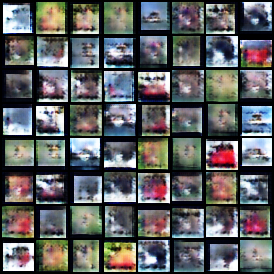
\includegraphics[width=\textwidth]{images/ex_2/try_1/epoch_20}
        \caption{Generated images from epoch 20 with transforms}
    \end{subfigure}
    \hfill
\end{figure}
In the final version, the images are just normalised to the same output format as the generated images, -1 to 1. \\


When implementing the optimisers, the same article\cite{brownlee_tips_2019} was referred in order to pick a suitable optimisation method and learning rate. Binary Cross-Entropy Loss is used since there are only two cases right and wrong for both generator and discriminator. The difference between the SGD and the Adam optimiser is that the Adam optimiser adapts its learning rates for each parameter depending  on the mean and variance of the gradient. \\
The training loop works through multiple batches per epoch. For each batch, first the gradients from the last training round are removed and then the discriminator is trained first and afterwards the generator. Note here that the discriminator is only trained every second iteration to prevent the discriminator being too strong. An early test run without that feature indicated: \\
\newline 
Saved images for epoch 60\\
Epoch [61/200] Dloss: 0.0799 Gloss: 6.4752\\
Saved images for epoch 130\\
Epoch [131/200] Dloss: 0.0523 Gloss: 6.2488\\

The generator loss was constantly oscillating between 5.5 and 7.8, not indicating any positive trend. The quality in the images also did not improve noticeably:
\begin{figure}[H]
    \centering
    \begin{subfigure}[t]{0.48\textwidth}
        \centering
        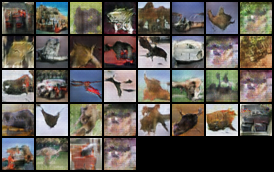
\includegraphics[width=\textwidth]{images/ex_2/try_1/epoch_80}
        \caption{Generated images from epoch 80}
    \end{subfigure}
    \begin{subfigure}[t]{0.48\textwidth}
        \centering
        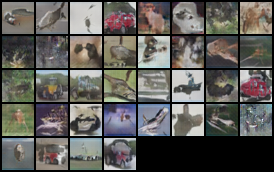
\includegraphics[width=\textwidth]{images/ex_2/try_1/epoch_140}
        \caption{Generated images from epoch 140}
    \end{subfigure}
    \hfill
\end{figure}
The training session was stopped, and the code modified to train the discriminator only half as much as the generator. However, the discriminator was still too strong. The epochs below indicate the generator losing confidence while the discriminator becomes more and more certain: \\
\newline 
Epoch [3/200] Dloss: 0.4726 Gloss: 2.1627\\
Epoch [30/200] Dloss: 0.2315 Gloss: 3.4251\\
\newline 
The training was stopped again, and the discriminator was only trained every third time. Which lead to the generator dominating. The compromise for the final training was to train the discriminator every second time but increase the dropout to 0.6, resulting in a more stable training process.\\
The following results are after 150 epochs of testing:

\begin{figure}[H]
    \centering
    \begin{subfigure}[t]{0.48\textwidth}
        \centering
        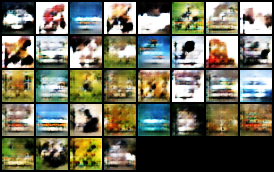
\includegraphics[width=\textwidth]{images/ex_2/try_2/epoch_10}
        \caption{Generated images from epoch 10}
    \end{subfigure}
    \begin{subfigure}[t]{0.48\textwidth}
        \centering
        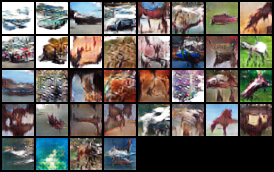
\includegraphics[width=\textwidth]{images/ex_2/try_2/epoch_30}
        \caption{Generated images from epoch 30}
    \end{subfigure}
    \hfill
\end{figure}


\begin{figure}[H]
    \centering
    \begin{subfigure}[t]{0.48\textwidth}
        \centering
        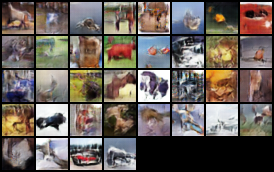
\includegraphics[width=\textwidth]{images/ex_2/try_2/epoch_40}
        \caption{Generated images from epoch 40}
    \end{subfigure}
    \begin{subfigure}[t]{0.48\textwidth}
        \centering
        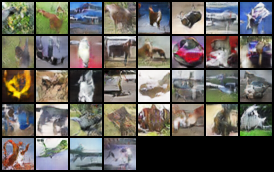
\includegraphics[width=\textwidth]{images/ex_2/try_2/epoch_70}
        \caption{Generated images from epoch 70}
    \end{subfigure}
    \hfill
\end{figure}



\begin{figure}[H]
    \centering
    \begin{subfigure}[t]{0.48\textwidth}
        \centering
        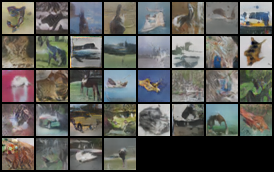
\includegraphics[width=\textwidth]{images/ex_2/try_2/epoch_100}
        \caption{Generated images from epoch 100}
    \end{subfigure}
    \begin{subfigure}[t]{0.48\textwidth}
        \centering
        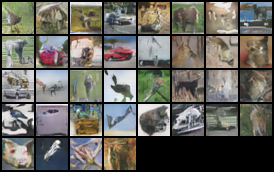
\includegraphics[width=\textwidth]{images/ex_2/try_2/epoch_150}
        \caption{Generated images from epoch 150}
    \end{subfigure}
    \hfill
\end{figure}
Obvious improvements can be made in the first thirty epochs. While the first bunch of images focuses on heavily distorted patterns, epoch 30 already features outlines and shapes that more closely resemble actual objects. 
Epoch 40 to 70 improve further and add more detail to the previously introduced shapes. Some images could resemble actual objects from the dataset like birds and dogs.
Epoch 100 to 150 offer little improvement. The biggest one is the colour which more closely resembles the desaturated nature of the dataset, which was missing in the previous epochs. However, the image quality only slightly improved. This is most likely related to the losses depicted in the figure above. \\
It can be observed that the generator is not improving in contrast to the discriminator, which is slightly improving. GANs are hard to train because if both parts do not remain in equilibrium, the training process can stagnate. That is why so much time was spent in correctly adapting the discriminator structure earlier. The current setup leads to the image quality plateauing at around 70-80 epochs, meaning the generator cannot keep up with the discriminator improving. The already referred article \cite{brownlee_tips_2019} actually recommends not implementing the fully connected layers at the end of the discriminator at all, so that might be a place to start optimising the process. As one previous try has shown, training the discriminator less often than the generator does not produce the intended effect.  Adjusting the learning rate of the discriminator to be lower could be a step to prevent the generator getting left behind. 

\begin{figure}[t]
        \centering
        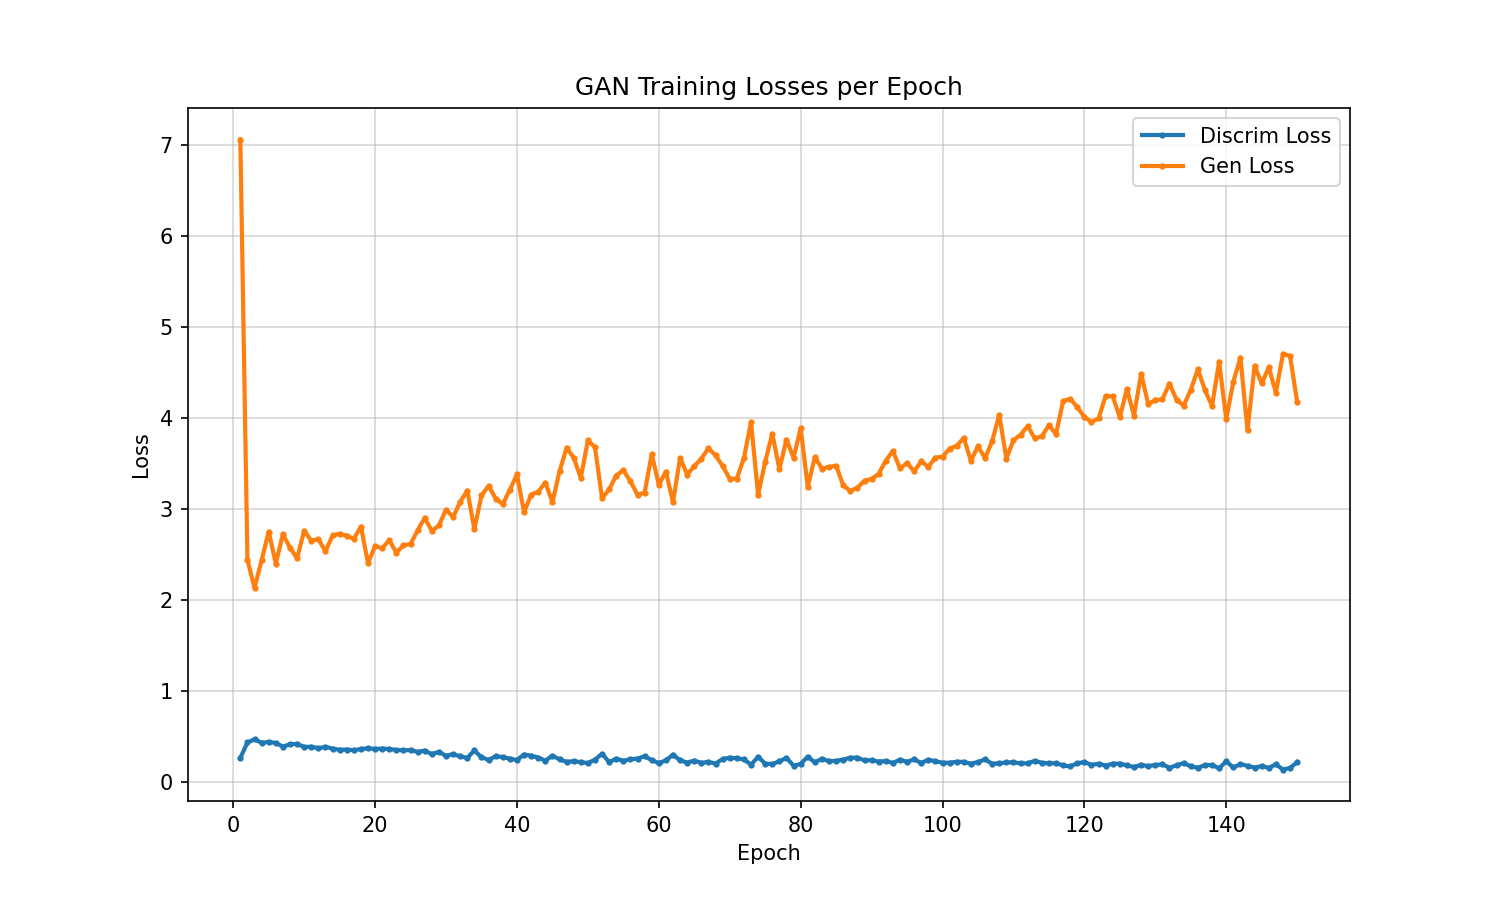
\includegraphics[width=\textwidth]{images/ex_2/try_2/training_losses_epoch}
        \caption{Losses during training}
    \end{figure}

\subsubsection{Training Implementation}
\textbf{Disclaimer}
Be aware that the model was trained on Google Colab just like the first lab session.
\lstinputlisting{scripts/ex_2/main.py}




















 